\section
[Single-server Queueing Process in Continuous Time]
{Construction of the Single-server Queueing Process in Continuous Time}
\label{sec:constr-gg1-queu}

In~\cref{sec:constr-discr-time} we modeled time as progressing in discrete `chunks': minutes, hours, days, and so on.
For given numbers of arrivals and capacity per period, we use the recursions~\cref{eq:31} to compute the departures and queue length per period.
However, we can also model time in a continuous way, so that jobs can arrive at any moment and have arbitrary service times. 
In this section, we consider a single-server FIFO queueing process in continuous time.


\opt{solutionfiles}{
\subsection*{Theory and Exercises}
\Opensolutionfile{hint}
\Opensolutionfile{ans}
}

Assume we are given the \recall{arrival process} $\{A(t); t\geq 0\}$, i.e., the number of jobs that arrived during $[0,t]$.
Thus, $\{A(t); t\geq 0\}$ is a \emph{counting process}.

From this arrival process, we can derive various other interesting concepts, such as the \recall{arrival times} of individual jobs.
Especially, if we know that $A(s) = k-1$ and $A(t) = k$, then the arrival time $A_k$ of the $k$th job must lie somewhere in $(s,t]$.
Thus, from $\{A(t)\}$, we can define\footnote{If we want to be mathematically precise, we must take $\inf$ rather than $\min$.
 However, in this book we do not want to distinguish between subtleties.}
\begin{equation}\label{eq:27}
 A_k = \min\{t: A(t) \geq k\},
\end{equation}
and set $A_0 = 0$.
Once we have the set of arrival times $\{A_k\}$, the set of \recall{inter-arrival times} $\{X_k, k=1, 2, \ldots\}$ between consecutive customers can be constructed as
\begin{equation}
 X_k = A_k - A_{k-1}.
\end{equation}

However, often the basic data consists of the inter-arrival times $\{X_k; k=1,2,\ldots\}$ rather than the arrival times $\{A_k\}$ or the arrival process~$\{A(t)\}$.
Then we construct the arrival times as
\begin{equation*}
 A_k = A_{k-1} + X_k,
\end{equation*}
with $A_0 = 0$.
From the arrival times $\{A_k\}$ we can, in turn, construct the arrival process $\{A(t)\}$ as
\begin{equation} \label{eq:2}
 A(t) = \max\{k: A_k \leq t\}.
\end{equation}
Thus, from the inter-arrival times $\{X_k\}$ it is possible to construct $\{A_k\}$ and $\{A(t)\}$, and from $\{A(t)\}$ we can obtain $\{A_k\}$ and $\{X_k\}$.


\begin{exercise}
Show that we can also define $A(t)$ as
\begin{equation}
 A(t) = \sum_{k=1}^\infty \1{A_k \leq t}.
\end{equation}
Thus, we just count all arrivals that occur up to and including time~$t$.
\begin{hint}
  What is $\1{A_k \leq t}$ if $A_k \leq t$? 
\end{hint}
\begin{solution}
For every $A_k \leq t$, we have that $\1{A_k \leq t} = 1$, and else the indicator is $0$. Hence, in the summation we count the number of times $A_k \leq t$. 
\end{solution}
\end{exercise}

\begin{extra}
Is it true that the following mappings are correct:
\begin{align*}
 A_k : \N \to \R, \quad{\text{job id (integer) to arrival time (real number)}}, \\
 A(t) : \R\to \N, \quad{\text{time (real number) to number of jobs (integer)}}?
\end{align*}
\begin{solution}
  Yes, it is true.
\end{solution}
\end{extra}

\begin{extra}
 What are the meanings of $A_{A(t)}$ and $A(A_n)$?
\begin{solution}
 $A(t)$ is the number of arrivals during $[0,t]$. Suppose that
 $A(t) = n$. This $n$th job arrived at time $A_n$. Thus, $A_{A(t)}$
 is the arrival time of the last job that arrived before or at time
 $t$. In a similar vein, $A_n$ is the arrival time of the $n$th
 job. Thus, the number of arrivals up to time $A_n$, i.e., $A(A_n)$,
 must be $n$.
\end{solution}
\end{extra}

\begin{extra}\clabel{ex:22}
 In view of the above, can $A(t)$ be defined as $\min\{k : A_k \geq t\}$ or as $\min\{k: A_k > t\}$?
\begin{hint}
Compare this to the definition in~\cref{eq:2}.
\end{hint}
\begin{solution}
 Suppose $A_3 = 10$ and $A_4 = 20$. Take $t=15$. Then
 $\min\{k : A_k \geq 15\} = 4$ since $A_3 < t=15 < A_4$. On the
 other hand $\max\{k : A_k \leq t\} = 3$. And, indeed, at time $t=15$, 3 jobs arrived, not 4. So defining $A(t)$ as $\min\{k : A_k \geq t\}$ is not OK. This example also shows that in general $A(t) \neq \min\{k : A_k > t\}$. So, neither definition is correct. 

\end{solution}
\end{extra}

The \emph{service times} of the jobs are given by the sequence $\{S_k\}$.
Typically we assume that the service times are i.i.d, and also independent of the arrival process $\{A(t)\}$.
With the arrival times and service times we can construct the \recall{waiting time in queue} $\{W_{Q,k}\}$ as seen by the jobs at the moment they arrive. 
From~\cref{fig:waitingtimegg1} it is evident that
\begin{equation}\label{eq:56}
 W_{Q,k} = [W_{Q,k-1} + S_{k-1}-X_k]^+.
\end{equation}
With this it is easy to compute the waiting times: from the initial condition $W_{Q,0}=0$ we can obtain $W_{Q,1}$, and then $W_{Q,2}$, and so on.

\begin{extra}
Explain that $W_{Q,k} = [W_{Q,k-1} + S_{k-1}-X_k]^+$. 
\begin{solution}
The waiting time of the $k$th arrival must be equal to the waiting time of the $k-1$th customer plus the amount of \recall{service time} required by job $k-1$ minus the time that elapses between the arrival of job $k-1$ and job $k$, unless the server becomes idle between jobs $k-1$ and $k$.
\end{solution}
\end{extra}

\begin{figure}[t]
 \centering

\begin{tikzpicture}[scale=1,
 open/.style={shape=circle, fill=white, inner sep=1pt, draw, node contents=},
 closed/.style={shape=circle, fill=black, inner sep=1pt, draw, node contents=}]
\draw (-1,0)--(12,0);

\draw 
node (c1) at (0,3) {}
node (Wk) at (1,2) [open, label={}]
(c1) to (Wk);

%\node[below] (Ak) at (1,-0.4) {$A_k$};
\draw[dotted] (1,0) -- (Wk) node[midway,fill=white,rotate=90] {$W_{Q,k-1}$};
\node (Sk) at (1,5) [closed, label={}];
\node (Ak1) at (5,1) [open, label={}];
%\node[above] at (4,0) {$D_k$};
%\draw[dotted,<->] (1, -0.25)--(3,-0.25) node[midway, fill=white] {$W_{Q,k}$};
%\draw[dotted,<->] (3, -0.25)--(6,-0.25) node[midway, fill=white] {$S_k$};
\draw[dashed] (1, 2)--(3,0); 

\draw[|-|]
node[left] (c1) at (1,-0.5) {$A_{k-1}$}
node[right] (c2) at (6,-0.5) {$D_{k-1}$}
(c1) -- (c2)
node[midway, fill=white] {$W_{k-1}$};

\draw[dotted] (Wk) -- (Sk) node[midway,fill=white,rotate=90] {$S_{k-1}$};
\draw[dashed] (Ak1) -- (6,0); % node[midway,fill=white,rotate=90] {$S_k$};

\draw[-] (Sk) to (Ak1);
\node (Sk1) at (5,3) [closed, label={}];
\draw[dotted] (Ak1) -- (Sk1) node[midway,fill=white,rotate=90] {$S_{k}$};
\draw[dotted] (5,0) -- (Ak1);
\draw (Sk1) -- (8,0);

\draw[|-|]
node[left] (c1) at (5,-1) {$A_{k}$}
node[right] (c2) at (8,-1) {$D_{k}$}
(c1) -- (c2)
node[midway, fill=white] {$W_{k}$};


\draw (9,2) -- (11,0);

\draw[dotted]
node (c1) at (9,0) [open, label={}]
node (c2) at (9,2) [closed, label={}]
(c1) -- (c2)
node[midway, fill=white, rotate=90] {$S_{k+1}$};

\draw[|-|]
node[left] (c1) at (9,-1.5) {$A_{k+1}$}
node[right] (c2) at (11,-1.5) {$D_{k+1}$}
(c1) -- (c2)
node[midway, fill=white] {$W_{k+1}$};

\draw[|-|]
node[left] (c1) at (1,-1.5) {$A_{k-1}$}
node[right] (c2) at (5,-1.5) {$A_{k}$}
(c1) -- (c2)
node[midway, fill=white] {$X_{k}$};
\end{tikzpicture}
\caption{Construction of the single-server queue in continuous time.
 The sojourn time~$W_{k}$ of the~$k$th job is the sum of the work in queue~$W_{Q,k}$ at its arrival epoch~$A_k$ and its service time~$S_k$; its departure time is then $D_k=A_k + W_k$.
 The waiting time of job $k$ is clearly equal to $W_{k-1}-X_{k}$.
 We also see that job~$k+1$ arrives at an empty system, hence its sojourn time $W_{k+1}=S_{k+1}$.
 Finally, the virtual waiting time process is shown by the lines with slope~$-1$.}
 \label{fig:waitingtimegg1}
\end{figure}




\begin{exercise}\clabel{ex:l-148}
 If $S\sim U[0,7]$ and $X\sim U[0,10]$, where $U[I]$ stands for the
 uniform distribution concentrated on the interval $I$, compute
 $\P{S-X\leq u}$, for $S$ and $X$ independent.
\begin{hint}
 This is elementary, hence it might appear trivial, but it's not\ldots In fact, I had a hard time finding a simple way to get the answer. It is good practice to try yourself before looking at the answer. Check also the previous problem, and make a drawing of the region over which you have to integrate.
\end{hint}
\begin{solution}
The joint density of $S$ and $X$ is given by
\begin{equation*}
 f_{XS}(x, s) = f_X(x) \cdot f_S(s) = \frac{1}{10} \1{0\leq x \leq 10}\cdot \frac 17 \1{0\leq s \leq 7},
\end{equation*}
since $X$ and $S$ are independent. 
Thus, 
\begin{equation*}
 \begin{split}
 \P{S-X\leq u} &= \E{\1{S-X\leq u}} = \frac{1}{70}\int_0^{10} \int_0^7 \1{s-x\leq u} \d s \d x \\
&= \frac{1}{70}\int_0^{10} \int_0^7 \1{s\leq x+u} \d s \d x.
 \end{split}
\end{equation*}

Now we need to chop up the domain of $\P{S-X\leq u}$, for which we use the figure below.

%\begin{figure}[ht]
\begin{center}
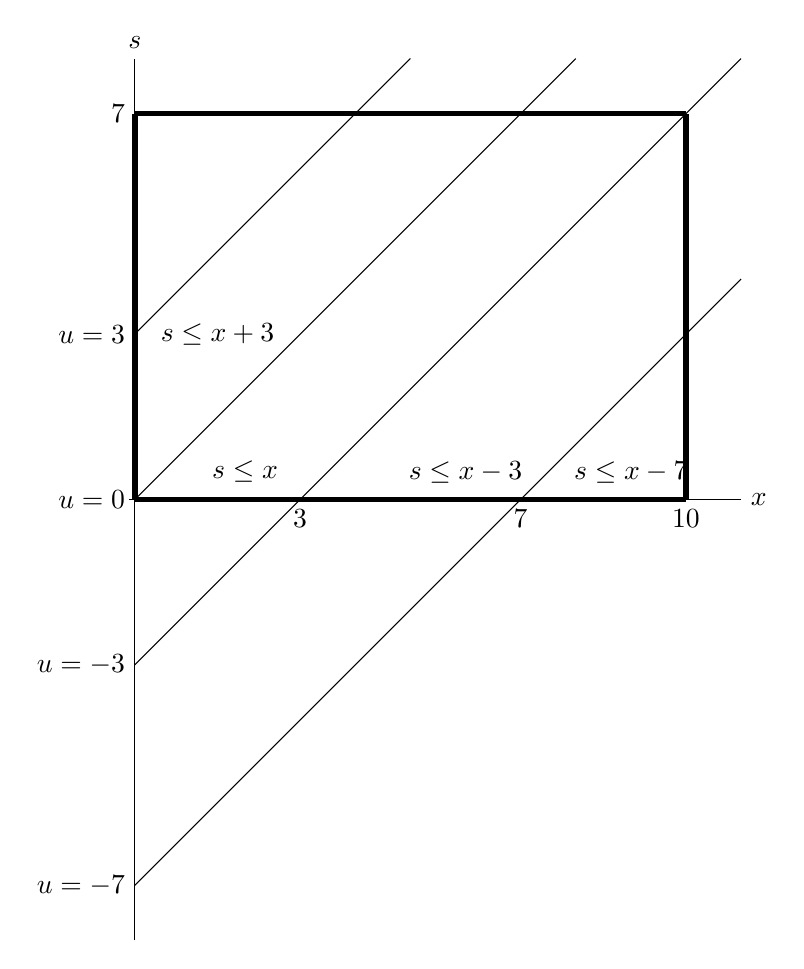
\begin{tikzpicture}[scale=0.7]
%\draw[[-{Triangle[open]},dotted] (0,10)--(8.5,10);
\draw (0,-8)--(0,8);
\node[right] at (11,0) {$x$};
\draw (-0.1,0)--(11,0);
\node[above] at (0,8) {$s$};
\draw[line width=0.7mm] (0,7)--(10,7);
\draw[line width=0.7mm] (10,0)--(10,7);
\draw[line width=0.7mm] (0,0)--(10,0);
\draw[line width=0.7mm] (0,0)--(0,7);
\node[below] at (10,0) {10};
\node[below] at (7,0) {7};
\node[below] at (3,0) {3};
\node[left] at (0,7) {7};
\draw (0,-7)--(11,4);
\node[left] at (0,-7) {$u=-7$};
\node at (9,0.5) {$s\leq x - 7$};
\draw (0,-3)--(11,8);
\node[left] at (0,-3) {$u=-3$};
\node at (6,0.5) {$s\leq x - 3$};
\draw (0,0)--(8,8);
\node[left] at (0,0) {$u=0$};
\node at (2,0.5) {$s\leq x$};
\draw (0,3)--(5,8);
\node[left] at (0,3) {$u=3$};
\node at (1.5,3) {$s\leq x+3$};
\end{tikzpicture}
\end{center}
%\caption{Computing the probability that $S-X\leq u$.}
%\label{fig:P_S_X}
%\end{figure}


It is clear that the indicated rectangle has no overlap with the set of points $(x,s)$ such that $s\leq u + x$ for $u<-10$. (To see this, draw the line $s=x-10$ in the figure.) At $u=-10$, the overlap is a single point, at $(10,0)$. Thus, 
\begin{equation*}
\P{S-X \leq u}=0, \quad \text{for } u\leq -10.
\end{equation*}

When $u\in[-10, -3]$ we need to integrate over the triangle that results from cutting the line $s=x+u$ with the rectangle. The area is 
\begin{equation*}
70\, \P{S-X \leq u}= \frac{(10+u)^2}2, \quad \text{for } -10 \leq u\leq -3,
\end{equation*}
where we multiply with $70$ to get the normalization right. 

When $u\in[-3, 0]$, we integrate over a parallelogram with base $3+u$ and height $7$ plus the triangle below the line $s=x-3$. The area is 
\begin{equation*}
70\, \P{S-X \leq u}= (3+u)7 + \frac{(10-3)^2}2=7u + \frac{91}2, \quad \text{for } -3 \leq u\leq 0.
\end{equation*}

For $u\in[0, 7]$, we integrate over the trapezoid that results from intersecting the set $\{(x,s) : x \leq s \leq s + u\}$ and the rectangle plus the parallelogram plus the triangle below the line $s=x-3$. The area is 
\begin{equation*}
70\, \P{S-X \leq u}= \frac{7^2}2 - \frac{(7-u)^2}{2} + 3\cdot 7 + \frac{49}2 = 7 u - \frac{u^2}2 + \frac{91}2, \quad \text{for } 0\leq u\leq 7.
\end{equation*}

Finally, for $u\geq 7$, the set $s\leq x+u$ covers the entire rectangle. Hence, 
\begin{equation*}
70\, \P{S-X \leq u}= 70, \quad \text{for } 7\leq u.
\end{equation*}

Given the amount of effort I had to put into getting this answer, I wanted to check it. So I went to Wolfram Alpha (which is a great site for symbolic computations), and typed this: 
\begin{verbatim}
\int_{0}^{10} \int_0^7 Boole[s<= x + u] ds dx,
\end{verbatim}
so, once you know \LaTeX\/ you can use Wolfram Alpha. Wolfram Alpha turned it to 
\begin{verbatim}
Integrate[Boole[s <= u + x], {x, 0, 10}, {s, 0, 7}]
\end{verbatim}
If you fill this in at Wolfram, you'll get the results that we obtained above in seconds, rather than in one hour or so (depending on your proficiency with carrying out integrals).
\end{solution}
\end{exercise}

The time job $k$ \emph{leaves the queue and moves to the server} is given by
\begin{equation*}
 \tilde A_k = A_k + W_{Q,k},
\end{equation*}
because a job can only move to the server after its arrival plus the time it needs to wait in queue.
Note that we here explicitly use the FIFO assumption.
Right after the job moves from the queue to the server, its service starts.
Thus,~$\tilde A_{k}$ is also the epoch at which the service of job~$k$ starts.

After completing its service, the job leaves the system.
Hence, the \recall{departure time of the system} is
\begin{equation*}
 D_k = \tilde A_{k} + S_k.
\end{equation*}
This in turn specifies the departure process $\{D(t)\}$ as
\begin{equation*}
 D(t) = \max\{k : D_k \leq t\} = \sum_{k=1}^\infty \1{D_k \leq t}.
\end{equation*}



The \recall{sojourn time}, or \emph{waiting time in the system}, $W_k$, is the time a job spends in the entire system.
With the above relations we see that
\begin{equation}
 W_k = D_k - A_k = \tilde A_{k} + S_k -A_k = W_{Q,k} + S_k,
\end{equation}
where each of these equations has its own interpretation. 


\begin{exercise}\clabel{ex:con-1}
 Explain that the following recursion for~$W_k$ is valid:
\begin{align}
 \label{eq:59}
 W_{Q,k} &= [W_{k-1} - X_k]^+, &
 W_{k} &= W_{Q,k} + S_k = [W_{k-1} - X_k]^+ + S_k,
\end{align}
from which follows a recursion for $D_k$:
\begin{equation}
 D_k = A_k + W_k.
\end{equation}
\begin{solution}
  Suppose $k$ arrives right after job $k-1$.
  Then job $k$ has to wait until job $k-1$ leaves, in other words, the service of job $k$ can start only after job $k-1$ leaves.
  Consequently, in this case, $W_{Q,k}=W_{k-1}$.
    If there is time $X_k$ between jobs $k$ and $k-1$, then job $k$ has to spend $X_k$ less in queue.
    This explains the first formula.
    The rest follows right away.
\end{solution}
\end{exercise}


\begin{extra}
 Assume that $X_1=10$, $X_2=5$, $X_3=6$ and $S_1 = 17$, $S_2=20$ and $S_3=5$, compute the arrival times, waiting times in queue, the sojourn times and the departure times for these three customers.
\begin{hint}
 The intent of this exercise is to make you familiar with the notation.

 BTW, such simple test cases are also very useful to test computer code.
 The numbers in the exercise are one such simple case.
 You can check the results by hand; if the results of the simulator are different, there is a problem.
\end{hint}
\begin{solution} Let's feed it to the computer. Mind that in Python (just like in C, and so on), arrays start at index 0, not at index 1. 
\begin{pyconsole}
X = [0, 10, 5, 6] 
S = [0, 17, 20, 5]
A = [0, 0, 0, 0]
for i in range(1, len(X)):
 A[i] = A[i-1] + X[i]

A

WQ = [0, 0, 0, 0]
for i in range(1, len(X)):
 WQ[i] = max(WQ[i-1] + S[i-1] - X[i], 0)

WQ

ST = [0,0,0,0]
for i in range(1, len(X)):
 ST[i] = WQ[i] + S[i]

ST

D = [0, 0, 0, 0]
for i in range(1, len(X)):
 D[i] = A[i] + WQ[i] + S[i]

D
\end{pyconsole}
 
\end{solution}
\end{extra}



\begin{extra}\clabel{ex:25}
 Assume that $X_k = 10$ minutes and $S_k = 11$ minutes for all
 $k$, i.e., $X_k$ and $S_k$ are deterministic and constant. What
 are $\lambda$ and $\mu$? Compute $A_k$, $W_k$, $D_k$ as functions of $k$. Then find expressions for $A(t)$ and $D(t)$.
\begin{solution}
 $\lambda=6$ per hour, and $\mu=60/11$ per hour. Note that
 $\mu < \lambda$. $A_0 = 0$, $A_1=10$, $A_2=20$, and so on. Hence,
 $A_k = 10k$. $W_{Q,0} = 0$, $W_{Q,1} = \max\{0 + 0-10,0\} = 0$.
 $W_{Q,2} = \max\{0+11-10,0\} =1$.
 $W_{Q,3} = \max\{1+11-10,0\} =2$. Hence, $W_{Q,k} = k-1$ for
 $k\geq1$. Thus, $W_k = k-1+11 = k + 10$ for $k\geq1$, and
 $D_k = 10k + k+10 = 11k+10$. Note that $W_k$ increases linearly
 as a function of $k$. All in all, $A(t) = \lfloor t/10\rfloor$, and $D(t) = \lfloor (t-10)/11 \rfloor$.
\end{solution}
\end{extra}


\begin{extra}
 Suppose that $X_k\in\{1,3\}$ such that $\P{X_k=1}=\P{X_k=3}$ and
 $S_k\in\{1,2\}$ with $\P{S_k=1}=\P{S_k=2}$. If $W_{Q,0}=3$, what are
 the distributions of $W_{Q,1}$ and $W_{Q,2}$? 
\begin{hint}
Use~\cref{eq:59}.
\end{hint}
\begin{solution} First find the distribution of $Y_k:=S_{k-1}-X_k$ so that we can write
 $W_{Q,k}=[W_{Q,k-1}+Y_k]^+$. Use independence of $\{S_k\}$ and $\{X_k\}$:
\begin{align*}
 \P{Y_k=-2} &=\P{S_{k-1}-X_k=-2} = \P{S_{k-1}=1, X_k=3} = \P{S_{k-1}=1}\P{X_k=3} = \frac14.
\end{align*}
Dropping the dependence on $k$ for ease, we get
\begin{align*}
 \P{Y=-2} &=\P{S-X=-2} = \P{S=1, X=3} = \P{S=1}\P{X=3} = \frac14,\\
 \P{Y=-1} &=\P{S=2}\P{X=3} = \frac14,\\
 \P{Y=0} &=\P{S=1}\P{X=1} = \frac14,\\
 \P{Y=1} &=\P{S=2}\P{X=1} = \frac14.
\end{align*}
With this
 \begin{align*}
 \P{W_{Q,1} = 1} &=\P{W_{Q,0} + Y= 1} = \P{3 + Y =1} = \P{Y=-2} =\frac14,\\
 \P{W_{Q,1} = 2} &= \P{3 + Y =2} = \P{Y=-1} =\frac14,\\
 \P{W_{Q,1} = 3} &= \P{3 + Y = 3} = \P{Y=0} =\frac14,\\
 \P{W_{Q,1} = 4} &= \P{3 + Y = 4} = \P{Y=1} =\frac14.\\
 \end{align*}
And, then
 \begin{equation*}
 \begin{split}
 \P{W_{Q,2} = 1} 
&=\P{W_{Q,1} + Y = 1} = \sum_{i=1}^4 \P{W_{Q,1} + Y = 1\given W_{Q,1}=i}\P{W_{Q,1}=i}\\
&=\sum_{i=1}^4 \P{i + Y = 1\given W_{Q,1}=i}\frac14
=\sum_{i=1}^4 \P{Y = 1-i\given W_{Q,1}=i}\frac14\\
&=\frac14\sum_{i=1}^4 \P{Y = 1-i} = \frac14(\P{Y = 0} + \P{Y=-1} +\P{Y=-2}) = \frac{3}{16}.
 \end{split}
 \end{equation*}

\begin{comment}
Typing the solution becomes boring\ldots, let's use the computer\footnote{To run this code, you need to install the lea package. This is a very useful package to help you with all kinds of probability experiments.}.
\begin{pyconsole}
import lea

W = 3
S = lea.vals(1, 2)
S
X = lea.vals(1, 3)
X

# This is WQ1
W = lea.max_of(W + S - X, 0, fast=True)
W

# This is WQ2
W = lea.max_of(W + S - X, 0, fast=True)
W
\end{pyconsole}
Great! Our handiwork matches with the computer's results. 
\end{comment}

\end{solution}
\end{extra}



\begin{exercise}\clabel{ex:l-149} 
Explain the following recursions for a single server queue: 
\begin{equation}
 \label{eq:45}
 \begin{split}
 A_k &= A_{k-1} + X_k, \\
 D_k &= \max\{A_k, D_{k-1}\} + S_k,\\
 W_k &= D_k - A_k.
 \end{split}
\end{equation}

\begin{solution}
 Of course, the service of job $k$ cannot start before it arrives.
 Hence, it cannot leave before $A_k + S_k$.
 Therefore it must be that $D_k \geq A_k +S_k$.
 But the service of job $k$ can also not start before the previous job, i.e.
 job $k-1$, left the server.
 Thus job $k$ cannot start before $D_{k-1}$.
 To clarify it somewhat further, define $S_k'$ as the earliest start of job $k$.
 Then it must be that $S_k' = \max\{A_k, D_{k-1}\}$---don't confuse the earliest start $S_k'$ and the service time $S_k$---and $D_k = S_k' + S_k$.
\end{solution}
\end{exercise}

The \recall{virtual waiting time process} $\{V(t)\}$ is the amount of waiting that an arrival would see if it would arrive at time $t$.
To construct $\{V(t)\}$, we simply draw lines that start at points $(A_k, W_k)$ and have slope -1, unless the line hits the $x$-axis, in which case the virtual waiting time remains zero until the next arrival occurs.


\begin{exercise}\clabel{ex:l-150}
 Provide a specification of the virtual waiting time process $\{V(t)\}$ for
 all $t$.
\begin{hint}Make a plot of the function $A_{A(t)}-t$. What is the meaning of $V(A_{A(t)})?$ What is
$V(A_{A(t)}) + A_{A(t)}-t$?
\end{hint}
\begin{solution}
 There is a funny way to do this.
 Recall from a previous exercise that if $A(t)=n$, then $A_n$ is the arrival time of the $n$th job.
 Thus, the function $A_{A(t)}$ provides us with arrival times as a function of $t$.
 When $t=A_{A(t)}$, i.e., when $t$ is the arrival time of the $A(t)$th job, we set $V(t) = V(A_{A(t)}) = W_{A(t)}$, i.e., the virtual waiting time at the arrival time $t=A_{A(t)}$ is equal to the waiting time of the $A(t)$th job.
 Between arrival moments, the virtual waiting time decreases with slope $1$, until it hits 0.
 Thus,
 \begin{equation*}
 V(t) 
= [V(A_{A(t)}) - (t-A_{A(t)})]^+= [W_{A(t)} + (A_{A(t)}-t)]^+.
 \end{equation*}
 The notation may be a bit confusing, but it is in fact very simple.
 Take some $t$, look back at the last arrival time before time $t$, which is written as $A_{A(t)}$.
 (In computer code these times are easy to find.)
 Then draw a line with slope $-1$ from the waiting time that the last arrival saw.
\end{solution}
\end{exercise}

Once we have the arrival and departure processes it is easy to compute the \recall{number of jobs in the system} at time $t$ as, cf.~\cref{fig:atltdt},
\begin{equation}\label{eq:14}
 L(t) = A(t) - D(t) + L(0),
\end{equation}
where $L(0)$ is the number of jobs in the system at time $t=0$; typically we assume that $L(0)=0$.
As in a queueing system, jobs can be in queue or in service, we distinguish between the number in the system $L(t)$, the number in queue $L_Q(t)$, and the number of jobs in service $L_s(t)$.

\begin{extra}\clabel{ex:97}
In~\cref{ex:25},  find an expression for $L(A_k-)$. 
\begin{solution}
Recall that $A(t) = \lfloor t/10\rfloor$, and $D(t) = \lfloor (t-10)/11 \rfloor$.
  Hence,
 \begin{equation*}
 L(A_k-) = k-1 - D(A_k-) = k- 1 - D(10k-) = k- 1 - \left \lfloor \frac{(10k-)-10}{11} \right \rfloor.
 \end{equation*}
 The computation is a bit tricky since sometimes arrivals and departures coincide. (Consider for instance $t=120$.)

From this example you can infer that it is necessary that the service rate is greater than the arrival rate, i.e., $\mu > \lambda$, for otherwise, the queue length keeps on increasing (in the long run).
\end{solution}
\end{extra}

In summary, starting from a sequence of inter-arrival times $\{X_k\}$ and service times $\{S_k\}$ we can obtain a set of recursions by which we can simulate a queueing process in continuous time. A bit of experimentation with Python (or R perhaps) will reveal that this is easy.

\begin{extra}
 Explain that if we know $\tilde A(t)$, i.e.
 the number of jobs that departed from the queue up to time $t$, then
\begin{align*}
 L_Q(t) &= A(t) - \tilde A(t), \\
L_s(t) &= \tilde A(t) - D(t) = L(t) - L_Q(t).
\end{align*}
\begin{solution}
  We defined $\tilde A(t)$ as the amount of people up to time $t$ that left the queue and moved to the server.
  It is then clear to see that the number of jobs in queue $L_Q(t)$ is equal to the number amount of jobs that have arrived, i.e., $A(t)$, minus the number of jobs that left the queue, i.e., $\tilde A(t)$.
  Using the same reasoning for $L_s(t)$,  the second line also follows.
\end{solution}
\end{extra}



\begin{figure}[ht]
 \centering
\begin{tikzpicture}[scale=0.9,
 open/.style={shape=circle, fill=white, inner sep=1pt, draw, node contents=},
 closed/.style={shape=circle, fill=black, inner sep=1pt, draw, node contents=},
 soldot/.style={color=blue,only marks,mark=*}
]

\def\rightend{14}
\def\top{7}
\path [clip] (-1,-1) rectangle (\rightend,\top);

\draw[->] (-1,0) -- (\rightend,0);
\draw[->] (-0.5,-0.5) -- (-0.5, \top);

% arrivals
\def\lastx{0}
\foreach \x [count=\y, remember=\x as \lastx] in {1,3,4, 7, 9, 18} { 
 \node at (\lastx, 0) [below] {$A_{\y}$};
 \node (a) at (\lastx,\y) [closed] {};
 \draw[dotted] (\lastx,0) -- (a); 
 \draw (a)-- (\x,\y) node[open, label={}]; 
}
% draw first arrival. Since I want the circle to be open, I draw it at
% the end.
\node at (0, 0) [open] {};
\node at (5.5, 4) [fill=white] {$A(t)$};


% departures
\def\lastx{5}
\foreach \x [count=\y, remember=\x as \lastx] in {6, 8, 10, 11, 13,15} { 
 \draw[dotted] (\lastx,\y) -- (\lastx,0); 
 \draw (\lastx,\y) node[closed, label={}] -- (\x,\y) node[open, label={}]; 
 \node at (\lastx, -0.5) [below] {$D_{\y}$};
}
\node at (5, 0) [open] {};
\node at (12, 5) [fill=white] {$D(t)$};
 
\draw[dashed, <->] (3,2.5)--node[midway, fill=white] {$W_3$} (8,2.5);
\draw[dashed, <->] (7.5,2)--node[midway, fill=white,rotate=90] {$L(t)$} (7.5,5);

\end{tikzpicture}

 
\caption{Relation between the arrival process $\{A(t)\}$, the departure process $\{D(t)\}$, the number in the system $\{L(t)\}$ and the waiting times $\{W_k\}$.
 In particular, $L(t)$ is the difference between the graphs of $A(t)$ and $D(t)$.
}
 \label{fig:atltdt}
\end{figure}




\begin{extra}
 Why don't we need a separate notation for $D_s(t)$, the number of jobs that departed from the server?
\begin{solution}
 Because $D_s(t) = D(t)$. Once customers leave the server,
 their service is completed, and they leave the queueing system.
\end{solution}
\end{extra}

\begin{extra}
 Is $\tilde A(t) \leq D(t)$ or $\tilde A(t) \geq D(t)$?
\begin{solution}
 All customers that left the system must have left the
 queue. Thus, $\tilde A(t) \geq D(t)$.
\end{solution}
\end{extra}



\begin{extra}
 Consider a multi-server queue with $m$ servers.
 Suppose that at some time~$t$ it happens that $\tilde A(t) - D(t) < m$ even though $A(t) - D(t) > m$.
 How can this occur?
\begin{solution}
 In this case, there are servers idling while there are still
 customers in queue. If such events occur, we say that the server
 is not work-conservative.
\end{solution}
\end{extra}


\begin{exercise}\clabel{ex:l-151}
 Show that $L(t) = \sum_{k=1}^\infty \1{A_k \leq t < D_k}$ when the system starts empty.
\begin{hint}
 Use Boolean algebra.
 Write, for notational ease, $A=\1{A_k \leq t}$ and $\bar A = 1- A = \1{A_k > t}$, and define something similar for $D$.
 Then show that $A - D = A \bar D - \bar A D$, and show that $\bar A D =0$.
 Finally sum over $k$.
\end{hint}

\begin{solution}
 \begin{equation*}
 \begin{split}
 L(t)
&= A(t) - D(t) \\
&= \sum_{k=1}^\infty \1{A_k \leq t} - \sum_{k=1}^\infty \1{D_k \leq t} \\
&= \sum_{k=1}^\infty [\1{A_k \leq t} - \1{D_k \leq t}].
 \end{split}
 \end{equation*}
 Write for the moment $A=\1{A_k \leq t}$ and
 $\bar A = 1- A = \1{A_k > t}$, and likewise for $D$. Now we can use
 Boolean algebra to see that
 $\1{A_k \leq t} - \1{D_k \leq t} = A-D = A(D+\bar D) -D = AD +
 A\bar D - D = A\bar D - D(1-A) = A\bar D - D \bar A$.
 But $D \bar A = 0$ since
 $D \bar A = \1{D_k \leq t} \1{A_k > t} = \1{D_k \leq t < A_k}$
 which would mean that the arrival time $A_k$ of the $k$th job would
 be larger than its departure time $D_k$. As $A \bar D = \1{A_k \leq t < D_k}$
 \begin{equation*}
 \begin{split}
 L(t)
&= \sum_{k=1}^\infty [\1{A_k \leq t} - \1{D_k \leq t}] \\
&= \sum_{k=1}^\infty \1{A_k \leq t < D_k}.
 \end{split}
 \end{equation*}
 Boolean algebra is actually a really nice way to solve logical puzzles.
 If you are interested, you can find some examples on my homepage.
\end{solution}

\end{exercise}

\begin{extra} Show that $L(A_k)>0 \implies A_k \leq D_{k-1}$.
\begin{hint} Use that $L(A_k)>0$ means that the system contains at least one job at the time of the $k$th arrival, and that $A_k \leq D_{k-1}$ means that job $k$ arrives before job $k-1$ departs.
\end{hint}
\begin{solution} In a sense, the claim is evident, for, if the system contains a job when job $k$ arrives, it cannot be empty.
 But if it is not empty, then at least the last job that arrived before job $k$, i.e., job $k-1$, must still be in the system.
 That is, $D_{k-1} \geq A_k$.
 A more formal proof proceeds along the following lines.
 Using that $A(A_k) = k$ and $D(D_{k-1})= k-1$,
 \begin{equation*}
 \begin{split}
 L(A_k) &> 0 \Leftrightarrow A(A_k) - D(A_k) > 0 \Leftrightarrow k - D(A_k) > 0 \Leftrightarrow k > D(A_k) \\
 &\Leftrightarrow k-1 \geq D(A_k) \Leftrightarrow D(D_{k-1}) \geq D(A_k) \Leftrightarrow D_{k-1} \geq A_k, 
 \end{split}
 \end{equation*}
 where the last relation follows from the fact that $D(t)$ is a
 counting process, hence monotone non-decreasing.
\end{solution}
\end{extra}

Define the number of jobs in the system as seen by the $k$th arrival as
\begin{equation}
 \label{eq:Lk}
 L(A_k-).
\end{equation}
Observe that we write $A_k-$, and not $A_k$.
As we are concerned with a process with jumps, we need to be quite particular about left and right limits at jump epochs.


\begin{exercise}\clabel{ex:55}
  With the recursions~\cref{eq:59} it is apparently easy to compute the waiting time (in queue), but it is less simple to compute the number of jobs in queue or in the system.
  In this exercise we develop an algorithm to compute the number of jobs in the system as seen by arrivals.  Explain why the following (algorithmic efficient) procedure works: 
 \begin{equation*}
 L(A_k-) = L(A_{k-1}-)+1 - \sum_{i= k-1 - L(A_{k-1}-)}^{k-1} \1{D_i< A_k}.
 \end{equation*}
% \hint{ Realize that $L_k = k - 1 - D(A_k)$. 
% what happens to job k-1?
% }
\begin{solution}
 Let $ L(A_{k}-)$, i.e., the number of jobs in the system as
 `seen by' job $k$. It must be that $L(A_{k}-)=k-1 - D(A_{k})$. To see
 this, assume first that no job has departed when job $k$
 arrives. Then job $k$ must see $k-1$ jobs in the system. In general,
 if at time $A_k$ the number of departures is $D(A_k)$, then the
 above relation for $L(A_k-)$ must hold. Applying this to job $k-1$ we get that $L(A_{k-1}-) = k-2 - D(A_{k-1})$. 

 For the computation of $L(A_k-)$ we do not have to take the departures
 before $A_{k-1}$ into account as these have already been
 `incorporated in' $L(A_{k-1}-)$. Therefore,
 \begin{equation*}
 L(A_k-) = L(A_{k-1}-) + 1 - \sum_{i= k-1 - L(A_{k-1}-)}^{k-1} \1{D_i< A_k}.
 \end{equation*}

 Suppose $L(A_{k-1})=0$, i.e., job $k-1$ finds an empty system at its
 arrival and $D_{k-1}>A_{k}$, i.e., job $k-1$ is still in the
 system when job $k$ arrives. In this case, $L(A_{k}-)=1$, which checks
 with the formula. Also, if $L(A_{k-1}-)=0$ and $D_{k-1}< A_k$ then
 $L(A_k-) = 0$. This also checks with the formula. 

\end{solution}
\end{exercise}


\begin{extra}
 In~\cref{ex:55}, why do we take $i=k-1-L(A_{k-1}-)$ in the sum, and not $i=k-2-L(A_{k-1}-)$?
\begin{solution}
 The reason to start at $k-1-L(A_{k-1}-)$ is that the number in the
 system as seen by job $k$ is $k-1 - D(A_k)$ (not
 $k-2-D(A_k)$). Hence, the jobs with index from
 $k-1-L(A_{k-1}-), k-L(A_{k-1}-), \ldots, k-1$, could have left the system
 between the arrival of job $k-1$ and job $k$.
\end{solution}
\end{extra}




\begin{extra}[Not obligatory] Try to extend the recursions~\cref{eq:45} to a situation in which one queue is
 served by two servers. 
\begin{hint} The problem is
 that in a multi-server queueing systems, unlike for
 single-server queues, jobs can overtake each other: a small job
 that arrives after a very large job can still leave the system
 earlier. After trying for several hours, I obtained an inelegant
 method. A subsequent search on the web helped a lot. The
 solution below is a modification of N. Krivulin, `Recursive
 equations based models of queueing systems'. 
\end{hint}
\begin{solution}
The recursions for the two-server system are this: 
 \begin{equation*}
 \begin{split}
 A_k &= A_{k-1} + X_k, \\
 C_k &= \max\{A_k, D_{k-2}\} + S_k,\\
 M_k &= \max\{M_{k-1}, C_k\}, \\
 D_{k-1} &= \min\{M_{k-1}, C_k\}.
 \end{split}
 \end{equation*}
 Here, $C_k$ is the completion time of job $k$, and $\{D_k\}$ is
 a sorted list of departure times. Thus, $D_k$ is the $k$th
 departure time; recall this is not necessarily equal to the
 completion time $C_k$ of the $k$th job (as jobs may overtake
 each other). To understand the other equations, we reason like
 this. By construction, $C_k > D_{k-m}$ (as $S_k >0$).
 Therefore, when we arrived at time $C_k$, $(k-m)$ jobs must have
 departed. Moreover, by construction, $M_k$ tracks the latest
 completion time of all $k$ jobs, hence, $M_{k-m+1}$ is the latest
 completion time of the first $k-m+1$ jobs. Therefore, if
 $C_k>M_{k-1}$, job $k$ must leave later than the latest of the
 jobs in $\{1,2,\ldots, k-1\}$. Hence, the latest departure time
 of the jobs in $\{1, 2, \ldots, k-1\}$ jobs must be
 $M_{k-1}$. If however, $C_k<M_{k-1}$, then job $k$ leaves
 earlier than the latest of the jobs in $\{1,2,\ldots, k-1\}$. As
 $C_k>D_{k-2}$, it must be that $C_k > M_{k-2}$, because
 $D_{k-2}$ is the latest departure of the jobs in
 $\{1,2,\ldots, k-2\}$, and this is also equal to $M_{k-2}$. As a
 consequence, if $C_k < M_{k-1}$, job $k$ is also the first job
 that leaves after $D_{k-2}$ ( provided of course that
 $C_{k+1} < C_k$). Thus, all in all
 $D_{k-1} = \min\{M_{k-1}, C_k\}$.

In an attempt to extend the above to $m>2$ servers, I came up with this scheme:
 \begin{equation*}
 \begin{split}
 A_k &= A_{k-1} + X_k, \\
 C_k &= \max\{A_k, D_{k-m}\} + S_k,\\
 M_k &= \max\{M_{k-m+1}, C_k\}, \\
 D_{k-m+1} &= \min\{M_{k-m+1}, C_k\},
 \end{split}
 \end{equation*}
 but it is not correct. Can you find a counterexample?
\end{solution}
\end{extra}





\opt{solutionfiles}{
\Closesolutionfile{hint}
\Closesolutionfile{ans}
\subsection*{Hints}
\input{hint}
\subsection*{Solutions}
\input{ans}
}

%\clearpage

%%% Local Variables:
%%% mode: latex
%%% TeX-master: "../companion"
%%% End:
